\begin{figure}[ht!]
	\centering
	\footnotesize

	\psfrag{x}[l][l] {$x$}
	\psfrag{y}[l][l] {$y$}

	\psfrag{A}[l][l] {$A(x_A,y_A)$}
	\psfrag{B}[l][l] {$B(x_B,y_B)$}
	\psfrag{C}[l][l] {$C(x_C,y_C)$}

	\psfrag{R2}[l][l] {$\mathbb{R}^2$}

	\psfrag{O}[l][l] {$\mathcal{O}$}

	\psfrag{Mx}[l][l] {$\mathcal{M}_x$}
	\psfrag{My}[l][l] {$\mathcal{M}_y$}

	\psfrag{M1}[l][l] {$\mathcal{M}_1$}
	\psfrag{M2}[l][l] {$\mathcal{M}_2$}

	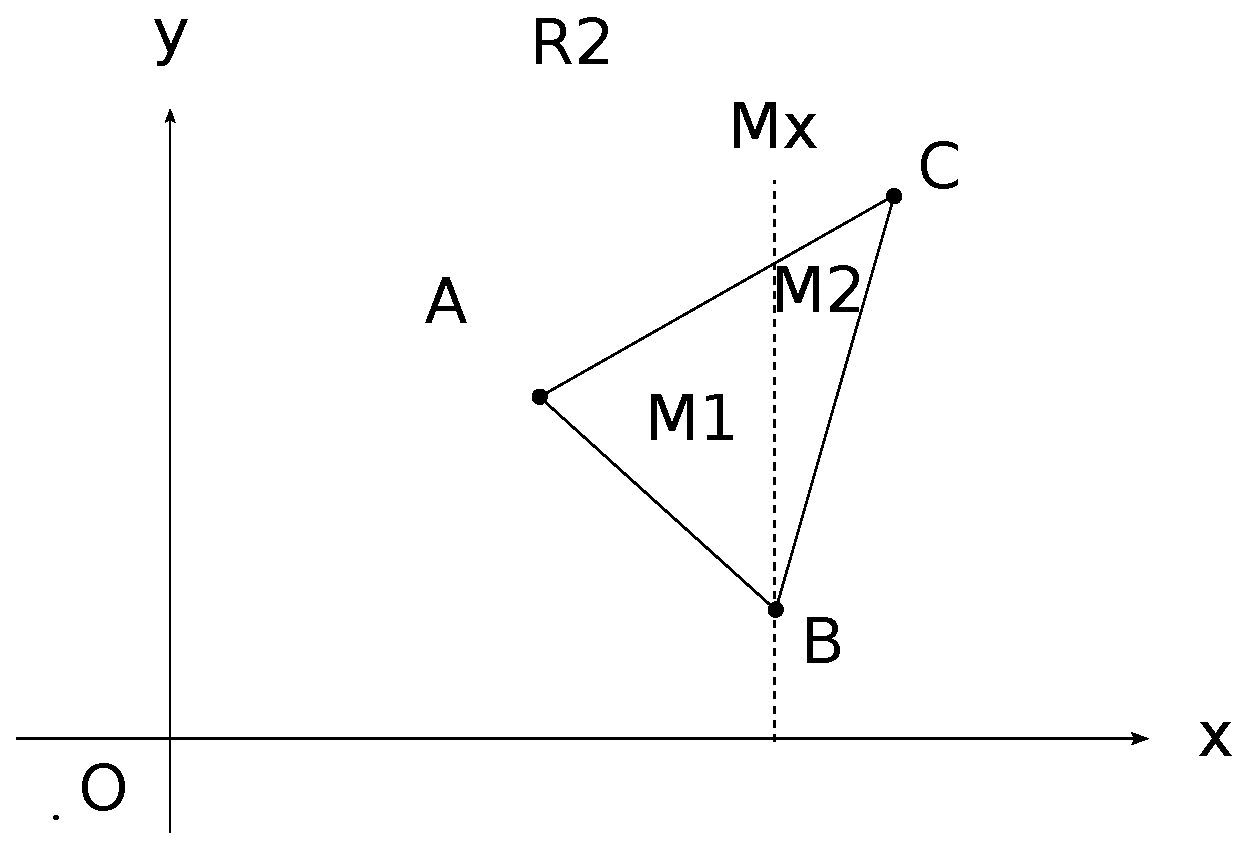
\includegraphics[width=0.8\textwidth]{setAinR2_Ax.eps}
	\caption{Set $\mathcal{M} \in \mathbb{R}^2$ where
		$\mathcal{M} = \mathcal{M}_{1} \cup \mathcal{M}_{2}$
		and split by $\mathcal{M}_x$.}
	\label{\LABEL}
\end{figure}
